\documentclass[11pt]{article}
\input{standalone-assets/preamble}
\renewcommand{\floatpagefraction}{0.80}
\renewcommand{\textfraction}{0.07}
\renewcommand{\topfraction}{0.92}
\renewcommand{\bottomfraction}{0.92}
\setcounter{topnumber}{4}
\setcounter{totalnumber}{6}
\raggedbottom
\emergencystretch=2em
\clubpenalty=10000
\widowpenalty=10000
\displaywidowpenalty=10000
\graphicspath{{figures/}{standalone-assets/}{tikz/}{./}}
\hypersetup{pdftitle={Seed and schedule sensitivity of mixture coupling in a contrastive autoencoder},pdfauthor={Zeyu Fu}}

\title{\textbf{Seed and schedule sensitivity of mixture coupling in a contrastive autoencoder}}
\author[1]{Zeyu Fu}
\affil[1]{State Key Laboratory of Trauma and Chemical Poisoning, Institute of Combined Injury,
Chongqing Engineering Research Center for Nanomedicine, College of Preventive Medicine,
Army Medical University, Chongqing, China\\
\texttt{fuzeyu09@gmail.com}}
\date{}

\begin{document}
\maketitle
\begin{abstract}
Late mixture coupling in a contrastive autoencoder is evaluated through representation geometry and an external branch-probability probe, rather than interpreting softmax-transformed latent coordinates as mixture allocation. A four-background descriptive grid at 200 epochs and a Setty-only 400-epoch sensitivity retain all three model seeds. On Setty, coupling changes branch-probe $R^2$ from $0.757/0.714/0.690$ to $0.678/0.662/-0.066$ at 200 epochs, whereas at 400 epochs both arms are positive: $0.767/0.624/0.729$ versus $0.651/0.518/0.667$. The sign heterogeneity at 200 epochs therefore does not persist across the two schedules. Revised nonself-neighbour purity decreases in all three stored Setty embeddings while retaining historical $K$-means labels. Global mixture occupancy and continuous coordinates are kept distinct: a former perplexity normalization by the 50-component truncation was inappropriate for a ten-dimensional softmax. A new complete-state matched coupling experiment gives lower edge survival and branch predictability in all three seed pairs. Executable invariant probes find unsynchronised query/key initial parameters and four query batch-normalisation calls per loss, but a single momentum and queue update per forward and an effective contrastive loss weight. The paired comparison establishes a seed- and schedule-dependent cost of coupling within this shared implementation, not the benefit of a correctly synchronised contrastive algorithm. They do not establish a bimodal outcome population, concentration equivalence, learned biological component identities, or superiority to an independently implemented contrastive method.
\end{abstract}

\section{Introduction}
Reconstruction, contrastive learning and mixture-density regularisation reward different properties of one encoder. Their combination requires controls that identify the intervention and report multiple representation endpoints. An organised embedding or a small effective component count alone cannot establish retention of a biologically relevant signal.

Contrastive learning provides a general framework for learning from relationships between examples. Momentum encoders and memory queues offer one way to supply comparison targets over many optimisation steps \cite{he2020momentum}; augmentation and projection choices also shape the learned representation \cite{chen2020simple}. In an implementation with stateful queues and batch normalisation, a nominally matched model seed is not the entire initial condition. The contents of those buffers, the random augmentation stream and the order of minibatches can influence subsequent updates. A coupling experiment is therefore strongest when its arms begin at the same complete algorithmic state, rather than merely sharing a seed label in an endpoint table.

Mixture regularisation supplies a different inductive preference. Variational Dirichlet-process mixtures can represent heterogeneous density with a finite computational truncation \cite{blei2006variational}. A neural encoder coupled to such a mixture may alter both the coordinates and the fitted mixture weights. The effective number of occupied components is then a property of the weights under a particular fit, not a direct count of cell types. Work linking adaptive mixtures and single-cell autoencoders motivates evaluating this interaction \cite{an2024scdac}. Our study examines one fixed contrastive autoencoder implementation; it does not claim to reproduce that method or isolate the contribution of contrastive learning from all other architectural choices.

The scientific question is whether adding the mixture term has a stable representation cost within this implementation. Stability has several meanings that should be separated. A paired difference can retain its direction across seeds while varying greatly in magnitude. An endpoint can change sign relative to a prediction baseline without producing a bimodal distribution of outcomes. A longer training recipe can improve an endpoint while also moving the intervention onset, making a pure duration explanation unavailable. These distinctions matter when a small experiment contains only three optimisation seeds: the individual values are informative, but they cannot identify the full distribution of possible training outcomes.

Single-cell haematopoiesis supplies a useful computational annotation for this question. Palantir provides branch probabilities describing inferred differentiation possibilities \cite{setty2019palantir}. Predicting those probabilities from a learned embedding tests whether a specific annotation remains locally accessible. It does not turn a computational annotation into experimentally traced lineage, and a negative cross-validated prediction score means performance below its baseline rather than demonstrated biological destruction. The probe complements a reference-neighbourhood measure that compares the embedding with PCA coordinates on the same held-out cells. Both can detect changes, but each depends on a defined representation of the task rather than an unrestricted notion of biological correctness.

Projection-based inspection answers a further question. UMAP can display structure in a low-dimensional view \cite{mcinnes2018umap}, but its coordinates and a chosen label-purity statistic need not preserve every relationship relevant to the branch probe. In the available archive, colouring uses historical clustering labels rather than curated cell identities. Such panels remain useful as descriptive checks when the label provenance and neighbour convention are explicit. They should be interpreted alongside the original-dimensional endpoints. In particular, a panel with relatively high clustering-label purity can still lose predictability of a continuous annotation, because the label partition and the branch probabilities encode different information.

We combine two forms of evidence. Historical four-background sweeps describe coupling and concentration at a fixed training recipe, and separately trained haematopoietic runs compare two total budgets. A new controlled experiment forks each seed's complete contrastive state after a common warmup, then applies coupled and uncoupled updates with matched minibatches, random streams and mixture-fitting samples. The new comparison holds the observed training window fixed and preserves complete model, optimiser and mixture states. It therefore directly tests coupling within the chosen algorithm while retaining the seed-level variability that motivates the study. It is not a contrastive-on versus contrastive-off experiment.

The contribution is a reproducible sensitivity analysis separating historical recipe comparisons from the paired intervention, and mixture occupancy from coordinate summaries. Complete branch states and individual endpoints bound the direction and variability of coupling effects under recorded conditions. They do not establish a universal weakness of contrastive learning or a biological interpretation of components.

\section{Materials and Methods}
Figure~\ref{fig:arch} identifies the shared encoder, contrastive routes,
mixture and decoder. Both coupling arms retain this machinery; their
difference tests the mixture coefficient within the recorded implementation.

\begin{figure}[!htbp]\centering
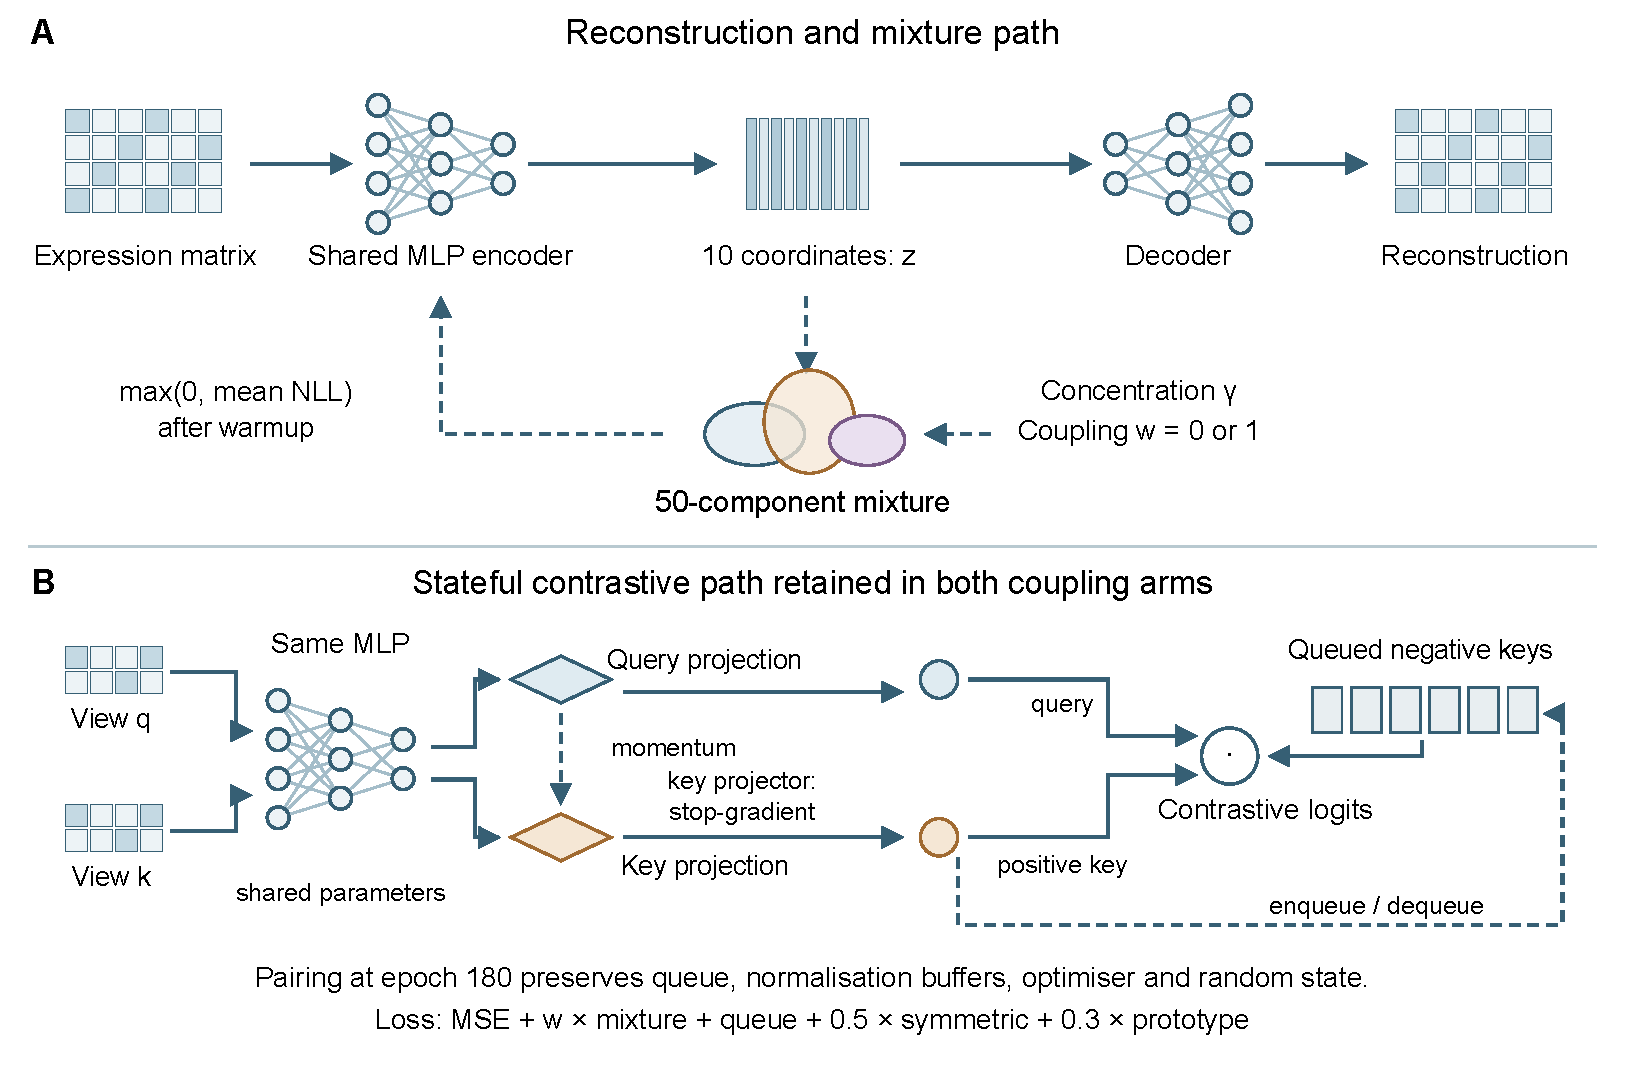
\includegraphics[width=\textwidth]{figures/architecture.pdf}
\caption{Computational paths in the contrastive coupling comparison.
A: expression passes through the shared MLP, ten unrestricted coordinates
and decoder. A 50-component diagonal mixture adds a weighted clamped
density penalty after warmup; dashed routes denote refits or state updates.
B: two augmentations use the same backbone. A query projector contrasts
positive keys with a queue; only key-projector parameters receive the
momentum update. The queue key-projector branch is stop-gradient; both
augmented views contribute backbone gradients through the symmetric term.
The full loss also
contains symmetric and prototype terms with coefficients 0.5 and 0.3.
At epoch 180, paired branches copy the model, queue, normalisation buffers,
optimiser and random state; only $w$ differs over twenty further epochs.
Matrix tiles and ellipses are computational objects, not observed cell types.}
\label{fig:arch}\end{figure}

\subsection{Implementation and intervention}
The model is an MLP autoencoder with momentum
contrastive machinery and a 50-component variational Gaussian mixture\cite{sklearn18bgm} on its
continuous ten-dimensional latent. The coupled and uncoupled arms retain
the same implementation and differ in the mixture coefficient $w$.
Reconstruction, augmentation, queue, momentum and batch-normalisation
behaviour are part of this fixed software recipe. There is no contrastive-off
factorial in these records, so they do not isolate the benefit of contrastive
learning itself.
Executable CPU probes of the frozen model code check initial query/key equality, a single forward momentum and queue transition, normalisation calls across forward and composite loss, and the contrastive-weight contribution for identical forward outputs. The protocol and data reside in \texttt{scripts/probe\_moco\_invariants.py} and \texttt{evidence/invariant-probe.json}. Synthetic four-row inputs make no optimiser update and are not additional biological experiments. The read-only archived-checkpoint audit resides in \texttt{scripts/audit\_saved\_states.py} and \texttt{evidence/checkpoint-metadata.json}. Both scripts run from this package: the first verifies SHA-256 identities of its bundled model and base-class sources, and the second reads archived checkpoints.

Mixture fitting begins after the 90\% warmup and repeats every ten epochs.
The named concentration comparison changes $\gamma$ at fixed $w=1$; it does
not test a continuum of concentration values.


\subsection{Exact loss and stateful contrastive route}
The encoder has widths $G$--256--128--10 and the decoder
10--128--256--$G$, with Mish hidden activations, batch normalisation
and zero dropout; the VAE and optional bottleneck are disabled.
With $z_i=f_\theta(x_i)$ and $\hat x_i=g_\phi(z_i)$, the batch objective is
\begin{align}
 \mathcal L_{\rm mix}&=\max\left\{0,-B^{-1}\sum_i
  \log\sum_{k=1}^{50}\pi_k\mathcal N(z_i;\mu_k,\Sigma_k)\right\},\\
 \mathcal L&=(BG)^{-1}\sum_i\|x_i-\hat x_i\|_2^2+w\mathcal L_{\rm mix}
   +\lambda(\mathcal L_{\rm queue}+0.5\mathcal L_{\rm sym}
   +0.3\mathcal L_{\rm proto}),\qquad\lambda=1.
 \label{eq:contrastive-objective}
\end{align}
The option named \texttt{kl} is a plug-in negative log density with a
lower clamp at zero, not a posterior KL divergence. It adds $10^{-10}$
inside logarithms of weights and precision factors; negative batch-average
NLL gives zero mixture gradient. Refits maximise the truncated-mixture
variational lower bound on fixed encoder outputs\cite{blei2006variational};
the fitted parameters are detached between refits. The prior is
stick-breaking with concentration $\gamma$, diagonal covariance,
mean precision 0.1, covariance regularisation $10^{-6}$, one $K$-means
initialisation, tolerance $10^{-3}$ and a 100-iteration ceiling.
Neither this density penalty nor the ten auxiliary prototypes identify
cell types\cite{xie2016deep,miller2014inconsistency}.

The query and key projectors map 10--10--128 through batch normalisation
and ReLU, followed by unit-length normalisation. A queue contains 4,096
negative keys, temperature is $\tau=0.2$, and only key-projector
parameters follow $\xi\leftarrow0.999\xi+0.001\psi$.
Both augmented views use the same backbone; this differs from a separate
momentum backbone. For the pre-enqueue bank $Q$,
\begin{equation}
 \mathcal L_{\rm queue}=-B^{-1}\sum_i\log
 \frac{\exp(q_i^\top k_i/\tau)}
 {\exp(q_i^\top k_i/\tau)+\sum_{u\in Q}\exp(q_i^\top u/\tau)}.
\end{equation}
This records the queue mechanism\cite{he2020momentum}; geometric
alignment alone does not certify downstream annotation retention\cite{wang2020alignment}.
The queue key-projector branch is stop-gradient; both augmented views
contribute backbone gradients through the symmetric term.
Enqueueing occurs once per forward.
For two query-projector outputs $h^1,h^2$, define
$S^{ab}_{ij}=(h_i^a)^\top h_j^b/\tau$. The symmetric term averages
$-S^{12}_{ii}+\operatorname{LSE}_j([S^{aa},S^{ab}]_{ij}
-[\operatorname{diag}(S^{aa}),\operatorname{diag}(S^{aa})]_{ij})$
over both views and cells ($b\ne a$). This is the recorded subtraction
of diagonal entries, including cross-view positives, rather than a
standard masked InfoNCE denominator. The prototype term is cross-entropy
over ten normalised learned prototypes, using each unaugmented cell's
own maximum-similarity prototype as its target.

Each augmentation applies independent Bernoulli feature retention 0.8,
then Gaussian noise of standard deviation 0.1 with batch-level probability
0.2, independent masking probability 0.1, and cell-wise scaling uniform
on $[0.8,1.2]$. Batch-normalisation buffers are stateful\cite{ioffe2015batch}:
one composite training loss invokes the query projector four times
(queue query, two symmetric views, unaugmented prototype) and the key
projector once. These counts, the initialisation discrepancy and the
loss-weight identity are checked by an independently rerun CPU probe.

\subsection{Data, evaluation and scope of replication}
The historical four-background panel comprises Setty haematopoiesis,
Dentate, pancreatic endocrinogenesis (Endo)\cite{bastidas2019endocrinogenesis}, and Lung. The Lung file GSE130148 is adult human lung from
unaffected regions of surgical resections, not a lung-development cohort
\cite{vieirabraga2019lung}. Historical runs cap each background at 3,000
cells and 3,000 highly variable genes, use preprocessing and random cell-split
seed 42, and train seeds 0--2 with latent dimension 10 and mixture truncation
50. Normalisation and feature selection preceded the cell split. This is a
transductive representation experiment, not an independent-patient prediction
study. The historical training batch size is 128. A model seed is not a donor,
and biological state identity is not identified by these runs.
Model seeds quantify optimisation variability; cells, overlapping
splits and repeated scores are not independent biological replicates.
The distinction prevents single-cell pseudoreplication\cite{zimmerman2021pseudoreplication};
computational uncertainty is conditional on the selected seeds and
training recipe\cite{bouthillier2021variance}.

The original descriptive grid has four backgrounds, three seeds, four
coupling values $w\in\{0,0.5,1,2\}$ and two concentration values
$\gamma\in\{0.02,1\}$, with the other axis held at 1. Its 72 records include
12 duplicate operating-point specifications: $w=1$ and $\gamma=1$ specify the
same configuration. The 400-epoch Setty sensitivity has nine records, of
which the $\gamma=1$ records repeat the $w=1$ specification. These are not
additional independent replications. A 90\% warmup moves from epoch 180 to
360 when the total budget doubles; both intervention onset and duration
therefore change.

Edge survival is a reference-graph diagnostic against the same held-out
cells' PCA-50 representation. It is not a cell-type or trajectory accuracy
measure. Reachability can remain one for a connected but rearranged graph.
Setty alone supplies Palantir branch probabilities for a five-fold $k$NN
regression probe, reported as $R^2$ at $k=15$\cite{setty2019palantir}.
These computed probabilities are an external computational annotation,
not prospective lineage tracing. A negative $R^2$ means worse prediction
than the fold-specific constant baseline; it does not establish biological
lineage destruction. A second historical branch score need not agree with
this local probe.

The latent $z\in\mathbb R^{10}$ is unconstrained. Applying softmax produces
ten coordinate weights, not fifty mixture responsibilities. The revised
RAAG-v2 scorer marks native-allocation scores as \texttt{non\_native} and
serializes their values as null. Softmax-coordinate coherence and perplexity
remain explicitly named coordinate diagnostics and do not support allocation
or cell-state claims. Gaussian conditional probabilities, where available,
are computed instead as
\begin{equation}
 r_{ik}=\frac{\pi_k\mathcal N(z_i;\mu_k,\Sigma_k)}
 {\sum_{j=1}^{50}\pi_j\mathcal N(z_i;\mu_j,\Sigma_j)}.
\label{eq:responsibility}
\end{equation}
These plug-in conditional probabilities are distinct from both the raw latent
and a full variational posterior over assignments.

UMAP panels use the 450 stored Setty test cells and the historical labels
0--9 produced by a $K$-means fallback. They are not curated cell-type labels.
The revised \texttt{umap-knn15-nonself-v2} purity uses each point's first 15
nonself neighbours. The former generator inadvertently omitted the first
nonself neighbour and included the sixteenth; the corrected-neighbour analysis rescores the unchanged
coordinates. Panel axes are independent UMAP coordinates without physical
units\cite{mcinnes2018umap}. Neither appearance nor label purity establishes
lineage recovery.

All new analyses are exploratory. The reporting and statistical interpretation were revised after inspecting the historical results; no prospective confirmatory significance is claimed. Per-seed values and paired contrasts remain visible.

\subsection{New common-state coupling protocol}
The new controlled Setty comparison uses seeds 0--2, 2,100 training cells,
450 held-out cells and 16 complete batches of 128 per epoch. Each seed
trains one 180-epoch warmup with an unfitted mixture. The complete registered
model state, including queue and batch-normalisation buffers, AdamW tensors
and NumPy/CPU/CUDA random states is saved, then deep-copied into $w=0$ and
$w=1$ branches. A discarded warmup-boundary update must produce identical
model and optimiser hashes across those branches. Precomputed epoch
permutations specify identical batches and fitting subsets. Each branch
then runs twenty epochs with refits at zero-indexed epochs 180 and 190.
The mixture coefficient is constant after onset; this implementation does
not use an annealing ramp. The optimizer uses learning rate $10^{-3}$,
weight decay $10^{-5}$ and gradient clipping 10, with no early stopping.
Mixture fitting uses 50 diagonal components, concentration 1, fixed
initialisation seed 42 and deterministic private jitter. All six endpoints
retain the complete encoder, optimiser, last installed mixture and an
additional full-training-set terminal observer. This experiment uses the
recorded contrastive implementation without changing momentum or queue
semantics. It isolates coupling within that code path, not the contribution
of contrastive learning as a separate factor.
AdamW applies decoupled weight decay\cite{loshchilov2019decoupled},
which is not an extra $L_2$ term in Eq.~\ref{eq:contrastive-objective}.
The branch probe uses distance-weighted $k$NN and five shuffled folds
(seed 42) of the 450 held-out cells; $R^2$ is averaged uniformly over
branch outputs and then over folds. These folds train the diagnostic
regressor, not the encoder. For the three matched seed differences we
report the arithmetic mean, sample standard deviation (denominator two),
and the three leave-one-seed-out means. None is a donor confidence
interval or a new biological replication. This sensitivity reuses all
saved endpoint scores without new neural updates or mixture fitting.

\section{Results}
\subsection{Setty branch prediction changes with seed and schedule}
Figure~\ref{fig:branch} and Table~\ref{tab:branch} provide the central result.
At 200 epochs, one coupled seed is slightly negative while two remain positive.
At 400 epochs all three coupled seeds are positive and all remain below their
own uncoupled counterpart. The largest 200-epoch loss is therefore not a
stable seed-specific failure across these two schedules. The repeated seed
numbers do not make the two budgets a continuation experiment: models are
trained independently and warmup is moved from epoch 180 to 360.

\begin{table}[htbp]\centering
\caption{Setty Palantir branch-probe $R^2$ at $k=15$. Columns are model seeds 0--2. Negative values indicate prediction below the cross-validation baseline, not proof that biological lineage was destroyed.}
\label{tab:branch}
\begin{tabular}{llrrr}\toprule
Budget & Coupling & Seed 0 & Seed 1 & Seed 2\\\midrule
200 & $w=0$ & 0.757 & 0.714 & 0.690\\
200 & $w=1$ & 0.678 & 0.662 & $-0.066$\\
400 & $w=0$ & 0.767 & 0.624 & 0.729\\
400 & $w=1$ & 0.651 & 0.518 & 0.667\\\bottomrule
\end{tabular}\end{table}

At 200 epochs, rescoring the same coupled latents with $k=10$ and $k=25$
keeps seeds 0 and 1 near $0.62$--$0.68$, whereas seed 2 remains no higher
than $0.005$. Thus the three tested neighbourhood choices preserve the
relative weakness of seed 2, although they do not preserve its exact sign.
A second historical Setty branch score moves from
$0.696/0.720/0.727$ to $0.712/0.812/0.788$ and does not reproduce the
negative local-prediction result. Neither metric is privileged as a complete
lineage certificate.
\begin{figure}[htbp]
\centering
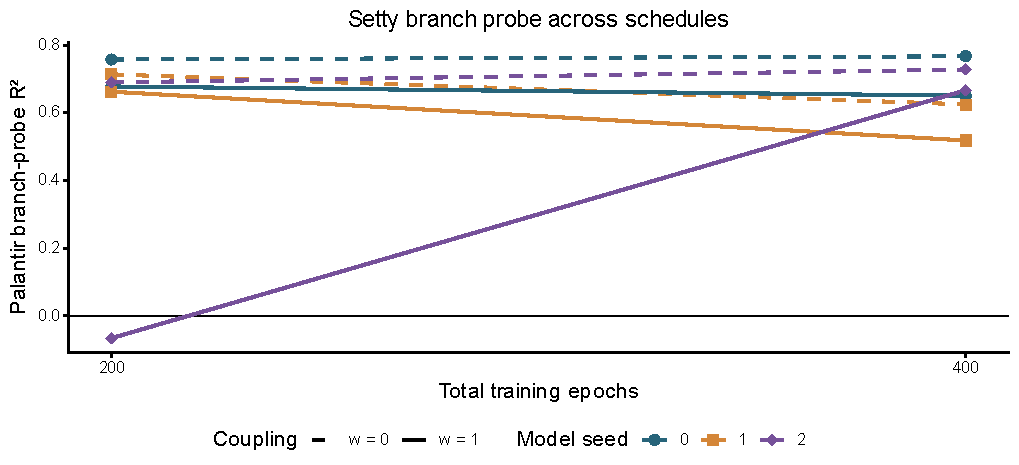
\includegraphics[width=0.96\textwidth,height=0.70\textheight,keepaspectratio]{figures/setty_palantir_seeds.pdf}
\caption{Historical Setty branch-probability predictability at two total
training budgets. The vertical axis is five-fold Palantir branch-probe
$R^2$ at $k=15$ on held-out cells; the horizontal axis is 200 or 400 training
epochs. Colour and shape jointly identify model seeds 0--2, while dashed
and solid lines identify $w=0$ and $w=1$, respectively, in one horizontal
shared key. The twelve points are individual run-level probe summaries,
without seed averaging or error bars. Lines connect separately trained
schedules, not checkpoints from a continuous trajectory. The zero line
marks the constant-prediction baseline. Warmup changes from epoch 180
to 360 with the total budget, so duration and intervention timing are
jointly varied. Negative $R^2$ and its seed dependence do not establish
lineage destruction or a bimodal population of outcomes.}
\label{fig:branch}
\end{figure}

\subsection{Neighbourhood costs and finite-mixture occupancy}
At 400 epochs the Setty edge score decreases for each seed:
$0.643\to0.611$, $0.612\to0.601$ and $0.611\to0.606$.
The historical 200-epoch four-background edge and effective-occupancy results
are shown in Figures~\ref{fig:edge} and \ref{fig:occupancy}. Their variation
across backgrounds motivates reporting the seed-level contrasts rather than
a universal benefit or harm. Effective occupancy is computed from global
mixture weights, not from softmax of latent coordinates. The 400-epoch Setty
values decrease from $28.9/35.4/35.2$ to $11.7/18.1/12.9$; corresponding
$K_{>1\%}$ values are $28/34/30$ and $15/21/19$.

These weights describe the last installed refit, which is not a terminal observer of the final encoder. No historical training covariance is imputed to recover missing responsibilities. The available concentration comparison is
descriptive and cannot establish equivalence or a universally inactive prior.
\begin{figure}[htbp]
\centering
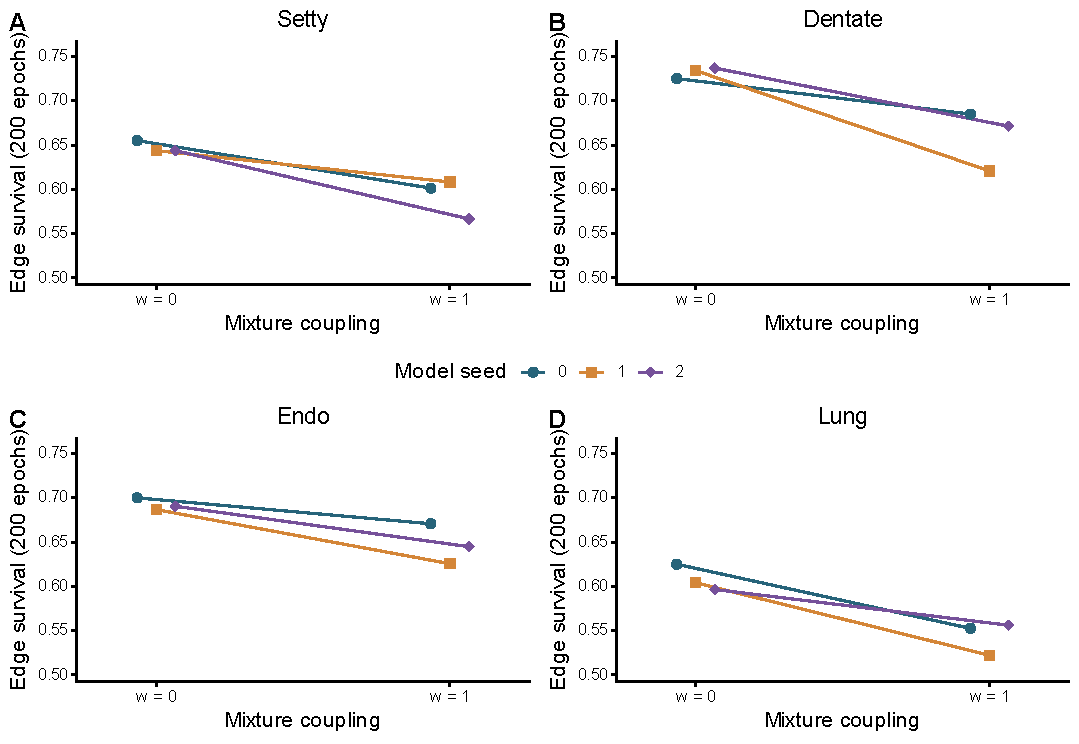
\includegraphics[width=0.96\textwidth,height=0.70\textheight,keepaspectratio]{figures/fourbg_edge_200.pdf}
\caption{Historical contrastive neighbourhood preservation at 200 epochs.
Panels A--D show Setty, Dentate, Endo and Lung on one common edge-survival
scale. The vertical score compares latent neighbours with PCA-50
neighbours of the same held-out cells. The horizontal axis contrasts
$w=0$ and $w=1$ at concentration $\gamma=1$; small offsets distinguish
seeds. Each panel contains six run endpoints connected within seeds
0--2. Colour and shape encode those seeds once in the full-width gutter
between panel rows. Lines show pairing rather than intermediate coupling
doses. Individual scores are displayed without seed aggregation or
error bars. These optimisation comparisons do not provide independent
biological replication or validate cell-state identities.}
\label{fig:edge}
\end{figure}
\begin{figure}[htbp]
\centering
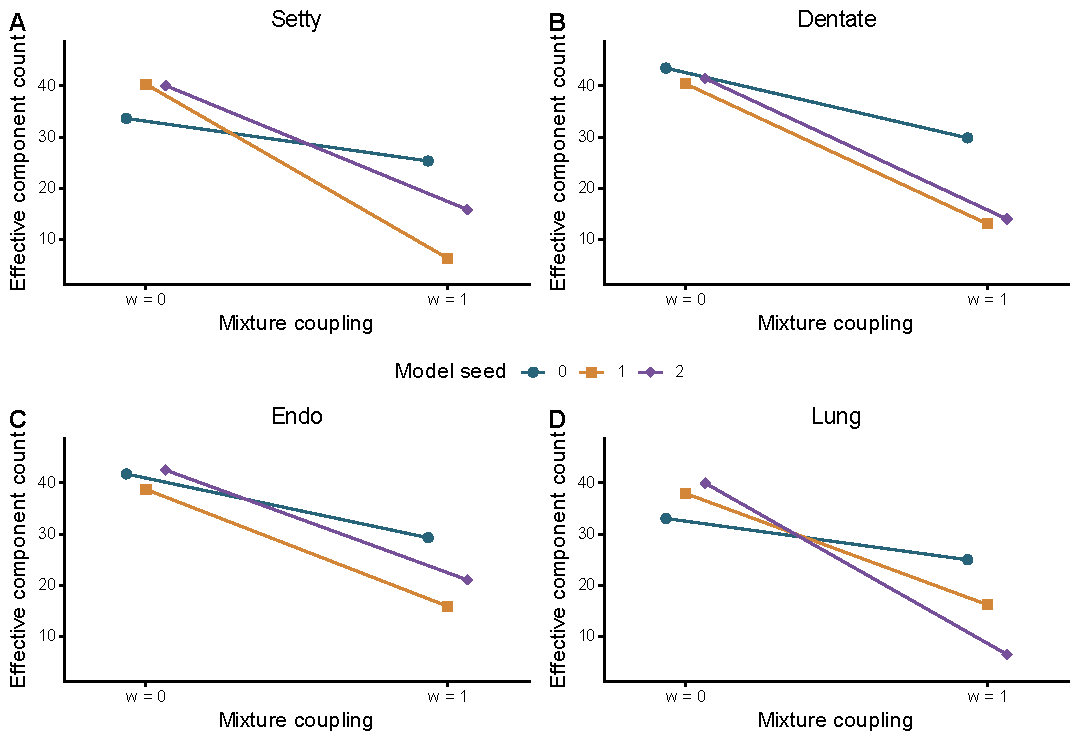
\includegraphics[width=0.96\textwidth,height=0.70\textheight,keepaspectratio]{figures/fourbg_components_200.pdf}
\caption{Historical contrastive effective occupancy of the last installed
mixture. Panels A--D map to Setty, Dentate, Endo and Lung, using one common
vertical scale. Effective occupancy is
$K_{\rm eff}=\exp[-\sum_k\pi_k\log\pi_k]$ from the 50 global mixture
weights; unlike $K_{>1\%}$ it does not threshold those weights.
At $\gamma=1$, each line pairs $w=0$ and $w=1$ endpoints for one model
seed after 200 total epochs. The shared horizontal legend between rows
jointly encodes seeds 0--2 by colour and shape, with slight horizontal
offsets to keep points visible. Six individual fit summaries per panel
are retained, without averaging seeds or adding error bars. These weights
come from the last training refit, not an observer fitted to the final
encoder. Occupancy depends on the estimator and refit time and does
not count independently established biological populations.}
\label{fig:occupancy}
\end{figure}

\subsection{Purity and coordinate diagnostics do not measure allocation}
Figure~\ref{fig:umap} shows the unchanged Setty UMAP coordinates.
Corrected nonself-neighbour purity is $0.7287/0.7622/0.7576$ at $w=0$
and $0.6314/0.7367/0.6196$ at $w=1$ (Table~\ref{tab:purity}). All three
paired differences remain negative after the scoring correction. These
historical $K$-means-label comparisons are descriptive; the better-looking
panel cannot identify which run retains Palantir predictability.

The former allocation argument used a transformed ten-coordinate latent.
At 400 epochs its perplexities range from 8.456 to 9.003. Dividing by the
50-component mixture truncation gives an invalid normalization; dividing
by ten gives fractions 0.846--0.900. Neither fraction is a measure of
50-component assignment uncertainty. Moreover, the old native-simplex guard
was inapplicable to these continuous latents: a false flag did not certify
nonuniform allocation. The revised scorer preserves this distinction.
A coordinate diagnostic exceeding a permuted-coordinate null does not make
it a biological or mixture allocation.
\begin{figure}[htbp]\centering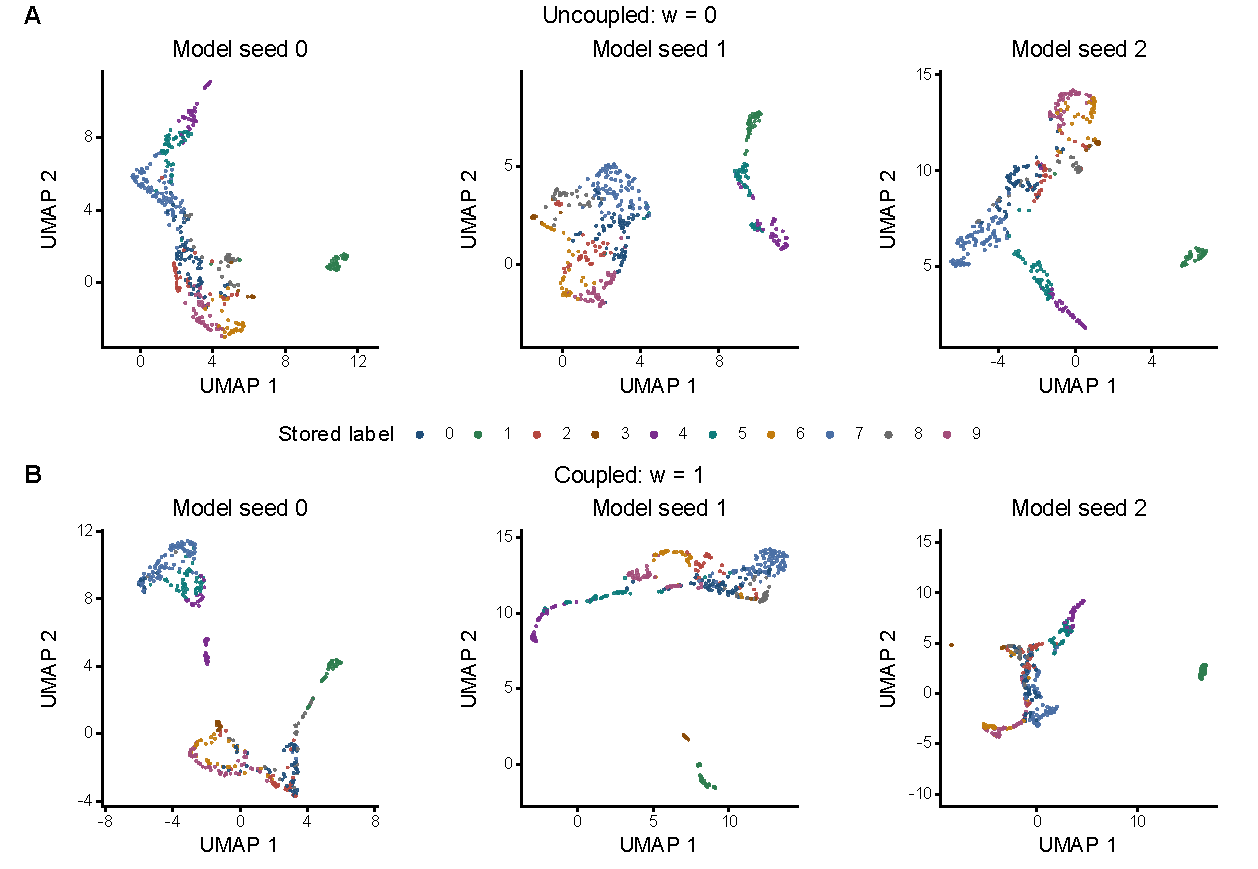
\includegraphics[width=0.96\textwidth,height=0.70\textheight,keepaspectratio]{figures/setty_umap.pdf}
\caption{Historical Setty contrastive projections at 200 epochs. Row A
shows $w=0$ and row B shows $w=1$ at $\gamma=1$; the three columns identify
model seeds 0, 1 and 2. Each tile plots all 450 stored held-out cells with
unchanged UMAP coordinates and no aggregation. The complete label key
appears once as a horizontal line between rows. Its colours identify
historical $K$-means assignments 0--9, not curated cell types or Gaussian
mixture components. Dimensionless UMAP axes have independent frames
across tiles and equal scaling within each tile, so projection orientation
and distance are not directly aligned between models.
Table~\ref{tab:purity} gives first-15-nonself-neighbour purity on these
coordinates. This descriptive projection and its label purity do not
identify which model retains the continuous Palantir annotation or
establish biological state identity.}\label{fig:umap}\end{figure}
\begin{table}[htbp]\centering\caption{Setty UMAP purity, first 15 nonself neighbours (v2), computed from unchanged coordinates. Labels are historical $K$-means assignments. Each panel contains 450 cells; the three columns are model seeds, not donors.}\label{tab:purity}\small\begin{tabular}{lcccc}
\toprule
Dose & seed 0 & seed 1 & seed 2 & mean $\pm$ s.d. \\
\midrule
$w=0$ & 0.729 & 0.762 & 0.758 & $0.750 \pm 0.018$ \\
$w=1$ & 0.631 & 0.737 & 0.620 & $0.663 \pm 0.065$ \\
\bottomrule
\end{tabular}
\end{table}

\subsection{Complete-state pairing confirms a coupling cost}
A new Setty experiment forks three complete contrastive warmup states into
coupled and uncoupled branches, with equal batches and twenty post-warmup
epochs (Figure~\ref{fig:paired}). The warmup-boundary model and optimiser
hash gates pass for all three pairs. Edge survival decreases from
$0.6487/0.6334/0.6553$ to $0.5463/0.5751/0.6190$ for seeds 0--2.
Branch-probe $R^2$ decreases from $0.7362/0.7535/0.7798$ to
$0.6696/0.0681/0.7197$. All paired directions agree, but the branch cost
is much larger for seed 1 than for the other two seeds. These are new
controlled trajectories, not replay of the historical endpoint table.
Independent differencing gives mean edge change $-0.0656$ (seed SD
$0.0337$) and branch change $-0.2707$ (seed SD $0.3591$).
Leave-one-seed-out means remain negative: $[-0.0803,-0.0473]$ for
edge survival and $[-0.3760,-0.0634]$ for branch $R^2$.
Thus the observed direction survives deletion of any one seed, while
the mean branch effect is strongly influenced by seed 1.
The experiment uses 10,560 unique scientific optimiser updates and six
discarded equality-probe updates. Complete last-refit and terminal-observer
parameters are saved; conditional probabilities are computed from their
Gaussian densities rather than from softmax coordinates.
\begin{figure}[htbp]\centering
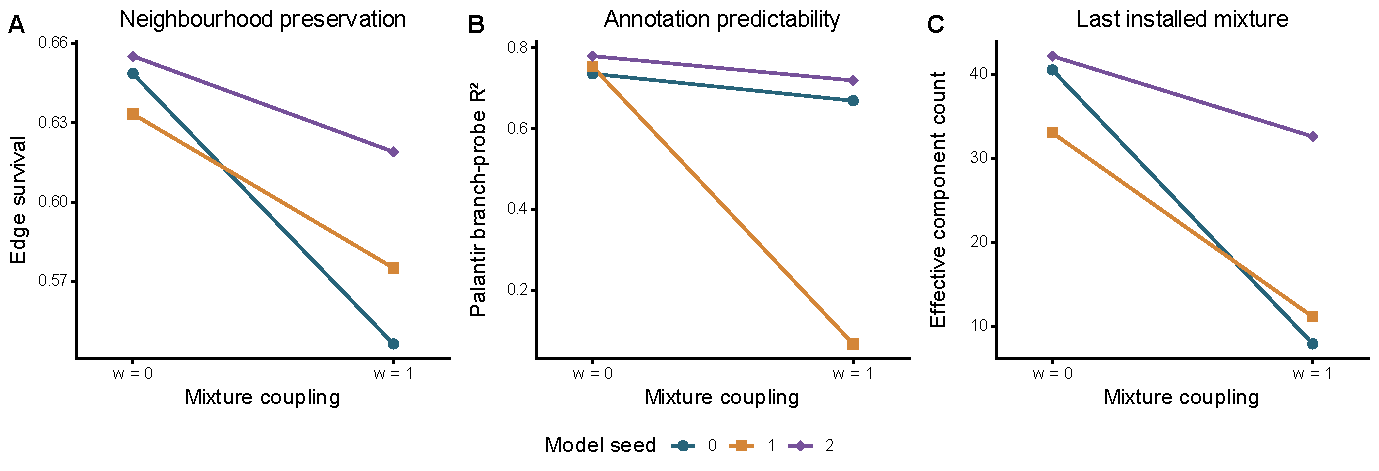
\includegraphics[width=\textwidth,height=0.70\textheight,keepaspectratio]{figures/matched_coupling.pdf}
\caption{Complete-state matched coupling on Setty. Panels A, B and C
respectively show held-out edge survival against PCA-50 neighbourhoods,
five-fold Palantir branch-probe $R^2$ at $k=15$, and effective occupancy
$\exp[-\sum_k\pi_k\log\pi_k]$ of the last installed training mixture.
The three distinct quantities retain separate vertical scales.
Horizontal positions compare $w=0$ with $w=1$ at $\gamma=1$; one shared
horizontal legend encodes seeds 0--2 by colour and shape.
Each line connects branches copied from the same seed's complete
180-epoch warmup state, including registered queue and normalisation
buffers, optimiser and random stream. Both branches receive twenty
further epochs with identical minibatches and refit samples at epochs
180 and 190. Panels A and B use the same 450 held-out cells; panel C
summarises the training fit rather than the terminal observer.
Each panel retains six individual endpoints without seed averaging or
error bars. Three paired histories quantify optimisation variability,
not biological sampling or the benefit of contrastive learning itself.}
\label{fig:paired}\end{figure}

\section{Discussion}
Mixture coupling decreases the Setty branch-probe score within each paired historical schedule, but the magnitude varies substantially across optimisation seeds. The negative score observed for one coupled seed at the shorter recipe does not persist at the longer recipe. The new controlled experiment also produces lower branch predictability and edge survival in all three coupled arms, while retaining strong heterogeneity in effect size. Together these results support an implementation-specific representation cost that is reproducible in direction under the tested pairings. They do not support a claim that all runs converge to the same outcome or that three observations identify distinct modes of a population distribution.

The new state-matched comparison improves attribution because the intervention begins from one complete warmup state per seed. Model parameters alone would not have been sufficient for this purpose. The contrastive queue, registered normalisation buffers, optimiser tensors and random-number state all belong to the training algorithm. Saving and restoring them ensures that the two branches begin with the same history. Shared minibatches and refit samples then remove important alternative explanations for an endpoint difference. The resulting effect is still conditional on the specified implementation, but it is more directly attributable to the mixture coefficient than a comparison between independently executed training recipes.

This design also clarifies what remains uncontrolled. Both arms retain the contrastive machinery, augmentations and reconstruction objective. Their difference therefore does not estimate the benefit of contrastive learning itself, nor does it establish superiority to a separately implemented contrastive method. A contrastive-off experiment would ask a different question and would need its own matching protocol. Moreover, a complete registered state does not certify that every intended algorithmic operation has the desired scientific effect. The experiment measures the behaviour of the recorded code path. Our executable single-forward probe finds one exact momentum update (maximum error below $10^{-6}$) and one four-key enqueue, with no extra enqueue in the loss. Across three synthetic initialisations, maximum query/key parameter discrepancies were $1.50$, $1.19$, and $1.21$; the key-copy operation was followed by another linear-layer initialisation. The query batch normaliser ran four times per composite loss versus once for the key. Changing \texttt{moco\_weight} from 1 to 0 on fixed forward outputs removed the computed contrastive composite (numerical residual $2.4\times10^{-7}$), but a zero weight does not disable forward state updates. Three archived initial checkpoints likewise had nonzero query/key differences; each 180-epoch warmup checkpoint recorded 11,520 query versus 2,880 key normaliser batches. Both mixture arms inherit these defects at the common branch state, so the paired coupling contrast remains meaningful within the recorded implementation. It does not show that a corrected momentum-contrast method would have the same effect. These probes do not substitute for retraining a corrected implementation.

The disagreement among representation diagnostics deserves substantive attention. A local branch-prediction score, a historical branch summary, neighbourhood overlap and projection purity can rank runs differently because they measure different retained structures. This is not resolved by selecting whichever score supports an expected conclusion. The branch probe uses a continuous computational annotation with cross-validation, whereas historical cluster-label purity summarises a partition of a two-dimensional projection. Neither quantity exhausts biological usefulness. Reporting the individual endpoints makes it possible to identify a tradeoff and avoids the false inference that a favourable plot has validated every downstream use of the embedding.

The longer historical recipe should likewise be interpreted as a joint schedule sensitivity. Doubling total epochs moves the ninety-percent warmup boundary, changes the duration of mixture exposure, and produces a separately trained model. It is not a continuation of the shorter checkpoint. Consequently, the disappearance of a negative seed score rules out treating that single endpoint as a fixed property of the seed across both recipes, but does not establish convergence or identify which schedule change caused the improvement. The new fixed-window pairing addresses the coupling contrast at one absolute onset; it does not retroactively convert the historical budget comparison into a controlled duration experiment.

Mixture occupancy provides useful complementary information only when its estimator is explicit. The reported effective count is calculated from global weights of the last installed fit. It is distinct from the uncertainty of cell-specific responsibilities and from the entropy of a softmax transformation of ten continuous coordinates. The new experiment saves complete training-mixture and terminal-observer parameters, allowing conditional probabilities to be derived without substituting coordinate weights for component assignments. Even these probabilities remain model-based quantities. A fifty-dimensional responsibility vector is mathematically appropriate to the fitted mixture, but its dimensions do not become validated biological populations merely because they sum to one.

The limits of replication constrain generalisation. Three model seeds quantify optimisation variability on the same processed data; they are not independent donors. The four descriptive backgrounds broaden computational context, but they do not provide a sampling design for population-level biological inference. Feature selection and normalisation were performed before the cell split, so the study concerns transductive representation analysis. The branch endpoint is available only for Setty. Different sample-level splits, externally validated annotations or preprocessing fitted solely to training samples could change the measured tradeoff. Those extensions would test generalisation while preserving the present experiment as a bounded observation.

Mixture coupling should be evaluated with complete algorithmic state and several defined endpoints. A paired direction remains informative when its unstable magnitude is visible. Future tests should preserve common-state branching, vary one schedule factor at a time and expand biological replication. The present controls support an implementation-specific cost of late coupling while retaining negative results and seed variability.

\section{Declarations}
\noindent\textbf{Data and code availability}\par\nobreak
The study-specific source repository is \url{https://github.com/PeterPonyu/contrastive-mixture-coupling}; the versioned research archive is \url{https://doi.org/10.5281/zenodo.22914495}. The archive contains the manuscript, vector figures, six paired endpoints, mixture parameters and responsibilities, batch-order arrays, source snapshots and executable invariant checks. Twelve model-state files are supplied separately within this archive for checkpoint-identity and warmup-state checks. The default saved-result analyses do not require checkpoints. Full historical neural training and raw-data score regeneration are not supplied. The repository README gives the dependency requirements, commands and checksums. Source studies and their data-access conditions are identified in Materials and Methods and the bibliography. Author-owned software is MIT licensed; the author's manuscript, figures, generated results and weights are CC BY 4.0. Third-party data and annotations retain their original terms.

\noindent\textbf{Ethics approval and consent}\par\nobreak
The reported work is a computational reanalysis of existing single-cell datasets; no new participant recruitment or animal experiment is described. Study-specific ethics review or exemption information, consent-to-participate information, and consent-for-publication declarations have not been established in this report. No ethics approval, exemption or consent status is inferred from dataset availability.

\noindent\textbf{Funding}\par\nobreak
This research received no funding.

\noindent\textbf{Author contributions}\par\nobreak
Zeyu Fu is the sole author of this manuscript. The affiliation and contact address are printed on the title page. The author is responsible for the manuscript and its computational analyses.

\noindent\textbf{Competing interests}\par\nobreak
The author declares no competing interests.

\noindent\textbf{Acknowledgements}\par\nobreak
The author acknowledges the researchers who made the cited source datasets and software available.

{\small\setlength{\bibsep}{0pt}\bibliographystyle{plainnat}\bibliography{standalone-assets/refs,extra}}
\end{document}
